%%%%%%%%%%%%%%%%%%%%%%%%%%%%%%%%%%%%%%%%%
% * <carreiravr@gmail.com> 2018-02-16T01:05:56.454Z:
%
% ^.
% * <carreiravr@gmail.com> 2018-02-16T01:05:53.114Z:
%
% ^.
% University Assignment Title Page 
% LaTeX Template
% Version 1.0 (27/12/12)
%
% This template has been downloaded from:
% http://www.LaTeXTemplates.com
%
% Original author:
% WikiBooks (http://en.wikibooks.org/wiki/LaTeX/Title_Creation)
%
% License:
% CC BY-NC-SA 3.0 (http://creativecommons.org/licenses/by-nc-sa/3.0/)
% 
% Instructions for using this template:
% This title page is capable of being compiled as is. This is not useful for 
% including it in another document. To do this, you have two options: 
%
% 1) Copy/paste everything between \begin{document} and \end{document} 
% starting at \begin{titlepage} and paste this into another LaTeX file where you 
% want your title page.
% OR
% 2) Remove everything outside the \begin{titlepage} and \end{titlepage} and 
% move this file to the same directory as the LaTeX file you wish to add it to. 
% Then add \input{./title_page_1.tex} to your LaTeX file where you want your
% title page.
%
%%%%%%%%%%%%%%%%%%%%%%%%%%%%%%%%%%%%%%%%%
%\title{Title page with logo}
%----------------------------------------------------------------------------------------
%	PACKAGES AND OTHER DOCUMENT CONFIGURATIONS
%----------------------------------------------------------------------------------------

\documentclass[12pt]{article}
\usepackage[english]{babel}
\usepackage[utf8x]{inputenc}
\usepackage{amsmath}
\usepackage{natbib}
\usepackage{graphicx}
\usepackage[colorinlistoftodos]{todonotes}
\usepackage{setspace}
\usepackage{float}
\usepackage{indentfirst}
\usepackage{mathtools}
\usepackage{hyphenat}
\usepackage{tcolorbox}
\hyphenation{E-di-to-ra}


\begin{document}

\begin{titlepage}

\newcommand{\HRule}{\rule{\linewidth}{0.5mm}} % Defines a new command for the horizontal lines, change thickness here

\center % Center everything on the page
 
%----------------------------------------------------------------------------------------
%	HEADING SECTIONS
%----------------------------------------------------------------------------------------

\textsc{\Large Universidade do Estado do Rio de Janeiro}\\[1.0cm] % Name of your university/college
\textsc{\large Redes Neuronais}\\[0.5cm] % Major heading such as course name
\textsc{\normalsize Roseli Wedemann}\\[0.5cm] % Minor heading such as course title

%----------------------------------------------------------------------------------------
%	TITLE SECTION
%----------------------------------------------------------------------------------------

\HRule \\[0.4cm]
{ \huge \bfseries \LARGE Notas de aula e Pesquisa pessoal}\\[0.4cm] % Title of your document
\HRule \\[1.5cm]
 
%----------------------------------------------------------------------------------------
%	AUTHOR SECTION
%----------------------------------------------------------------------------------------

\begin{minipage}{0.4\textwidth}
\begin{flushleft} \large
\emph{Autor:}\\
Victor Carreira % Your name
\end{flushleft}
\end{minipage}
~
\begin{minipage}{0.4\textwidth}
\begin{flushright} \large
\emph{Professora:} \\
Dra. Wedemann % Supervisor's Name
\end{flushright}
\end{minipage}\\[2cm]

% If you don't want a supervisor, uncomment the two lines below and remove the section above
%\Large \emph{Author:}\\
%John \textsc{Smith}\\[3cm] % Your name

%----------------------------------------------------------------------------------------
%	DATE SECTION
%----------------------------------------------------------------------------------------

{\large \today}\\[2cm] % Date, change the \today to a set date if you want to be precise

%----------------------------------------------------------------------------------------
%	LOGO SECTION
%----------------------------------------------------------------------------------------


\includegraphics[scale=0.5]{Imagens/logo_uerj.png}\\[1cm] % Include a department/university logo - this will require the graphicx package
 
%----------------------------------------------------------------------------------------

\vfill% Fill the rest of the page with whitespace

\end{titlepage}


\begin{abstract}
This work aims to publicate my neural network class notes from the discipline of professor Roseli Wedemann, among the period from August 2017 to January 2018 of the Stadual University of Rio de Janeiro, Brazil.
\end{abstract}

\section{Primeira aula: 09/08/2017 }
\onehalfspacing

Por quê o termo redes "neuronais"?\\
O termo neuronal se refere ao estudo de redes inspiradas nos neurônios que compõe o sistema cerebral.  Estes não tem relação com todos os neurônios que compõe o sistema nervoso central, mas compõem uma classe limitada de neurônios. 

A bibliografia utilizada neste curso, na ordem de maior para menor importância, é apresentada a seguir:

\begin{enumerate}
	\item Introduction to the theory of neuronal computation, J. Hertz, A. Krogh, R.G. Palmer, Lecture notes Vol. I, Santa Fe Institute, Studies in the science of complexity , Perseus Books.
	\item Neural networks: A comprehensive foundation, S. Haykin, Macmillan Publishing Co.
	\item Data Mining, A mineração de dados no Marketing, Medicina, Economia, Engenharia e Adminstração, Luis Alfredo Vidal de Carvalho, Editora Ciência Moderna.     
\end{enumerate}

\subsection{Introdução}

O cérebro humano pode realizar muitas tarefas melhor do que os sistemas de inteligência artificial \footnote{A abreviatura do termo ,IA,  é muitas vezes utilizada em diversas publicações na literatura específica e será adotado nestas notas de aula. }, por exemplo, no processamento de imagens.

O computador, por sua vez, realiza muito melhor tarefas aritméticas. 

\subsubsection{Aprendizado simbólico}

O aprendizado simbólico é nato do ser humano, durante a sua fase infante, e tem extrema importância para a aprendizagem, visto que a função simbólica que dá conta de todo o processo de pensamento. A simbolização inicia-se no momento da separação do bebê com a mãe, possibilitada pelo \textit{Complexo de Édipo}\footnote{Complexo de Édipo é o termo cunhado por Sigmund Freud em sua teoria de estágios psicossexuais do desenvolvimento para descrever os sentimentos de um menino: desejo pela mãe e ciúme e raiva em relação a seu pai.}, com a entrada de uma terceira pessoa, o pai, na função paterna. 

Segundo \citet{Ferreiro1999} o aprendizado simbólico responsável pela fala e escrita ocorre em 5 níveis, no qual o último representa a compreensão dos diferentes caracteres da escrita associados aos sons. Nesta fase, o infante consegue diferenciar o som de um caractere e de um fonema. E a partir dessa etapa, a criança se defronta com as dificuldades próprias da ortografia.

\subsubsection{Aprendizado Conexionista }

O conexionismo é uma teoria do conhecimento que se preocupa com todo o processo que aquisição e, por isso, tem uma proposta de esclarecer a aprendizagem e explicar a memória. O paradigma conexionista apresenta estreita relação entre aprendizagem e memória a medida que não pode haver um sem o outro \citep{Rossa2009}. 

\begin{figure}[H]
\centering
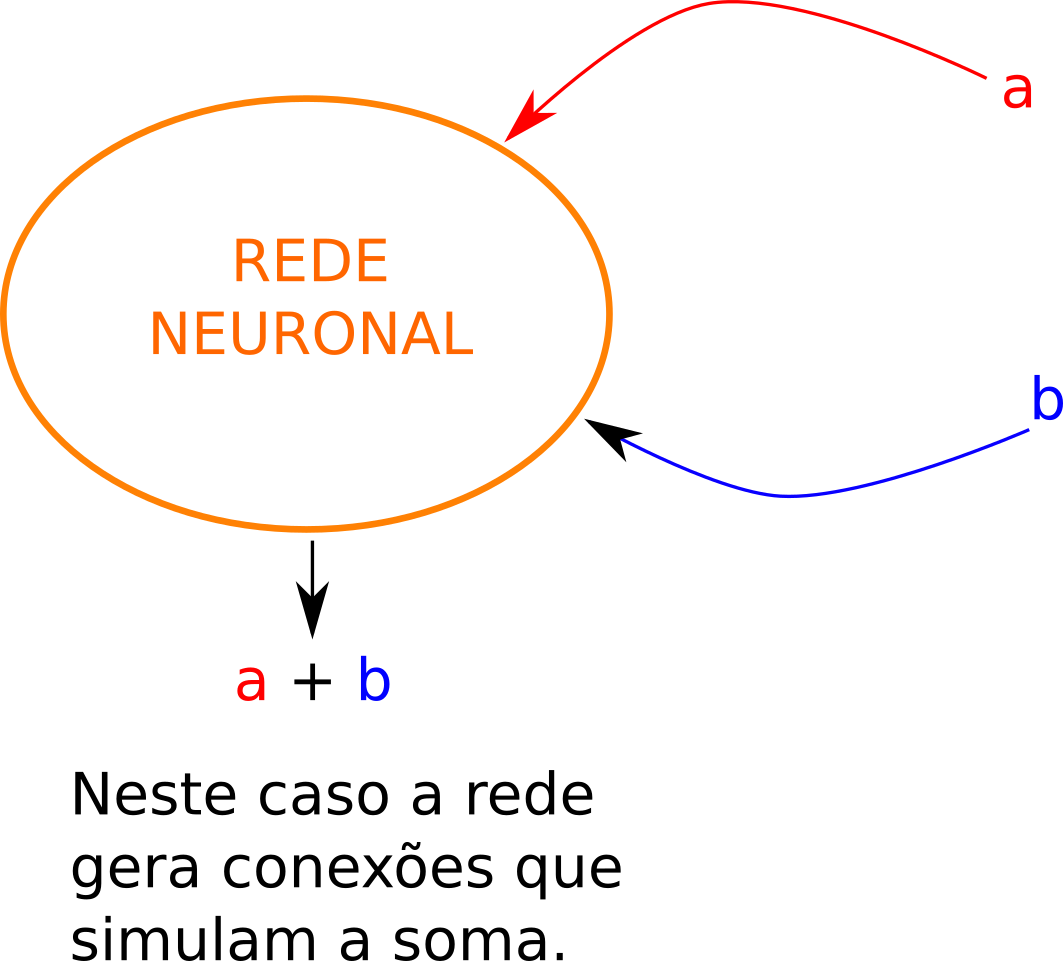
\includegraphics[width=0.5\textwidth]{Imagens/Fig1.png}
\caption{Modelo conexionista. A soma "a + b" é a soma de dois símbolos aprendidos em uma etapa anterior.}
\end{figure}

Diferentemente do modelo simbólico o modelo conexionista pega o símbolo "a" e "b" e gera a soma "a + b".

\subsubsection{Neurocomputação}

\subsubsection{Redes Criativas }

\subsubsection{Computação coletiva}

\begin{figure}[H]
	\centering
	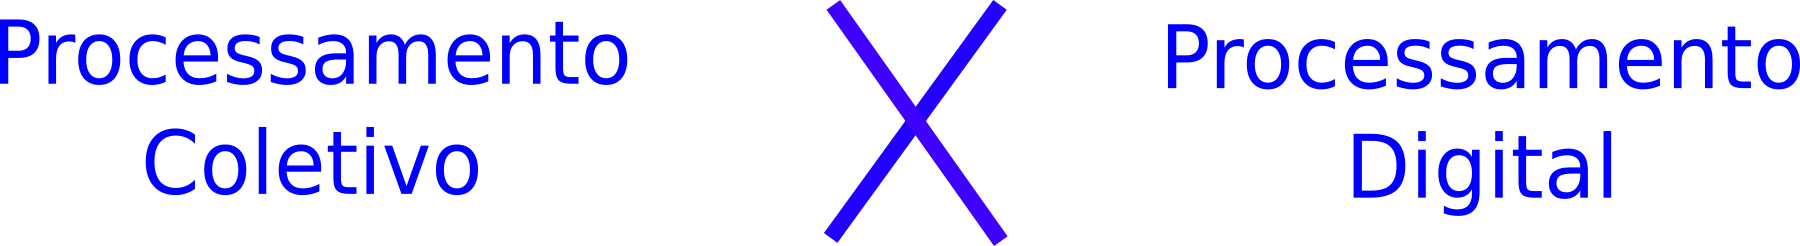
\includegraphics[width=1\textwidth]{Imagens/Fig2.png}
	\caption{Dois tipos de processamento.}
\end{figure}

O processamento distribuído realiza diversas tarefas em paralelo, a exemplo do cérebro, que realiza o processamento de imagens em paralelo com a respiração e os batimentos cardíacos . Já o processamento sequencial, nos computadores, realizam somente uma tarefa de cada vez. 

A computação em paralelo é uma forma de se tentar aproximar a capacidade de processamento do cérebro humano. Nossa evolução biológica convergiu o nosso cérebro para um tipo de processamento em paralelo.  

A grande vantagem da rede neuronal artificial é que ela tem a capacidade de resolver sistemas físicos não-lineares. Por exemplo, a evolução de sistemas no tempo como as colônias de formigas são alguns tipos de problemas que podem ser solucionados através de redes neuronais artificiais. 

Células nervosas morrem todos os dias e a performance do cérebro não é significativamente afetada o que confere robustez e tolerância. Os ajustes e flexibilidades ocorrem conforme o aprendizado. Outra característica fundamental do cérebro humano é que ele consegue ajustar informações que são nebulosas, probabilísticas, ruidosa e inconsistente. Realiza tarefas em paralelo além de ser compacto pequeno e dissipa pouca energia. 

Desta maneira, a computação neuronal é uma alternativa a computação de \textit{von Neumann} ou a paradigma de \textit{von Neumann}\footnote{Programação sequencial} comumente usada em computadores.   Desta maneira, as RNAs\footnote{Redes Neuronais Artificiais} são inspiradas na neurociência, muito embora não sejam realísticas em termos biológicos. E seus métodos matemáticos advém da \textit{Física Estatística}, que é um ramo da Física que se atém ao desenvolvimentos de técnicas matemáticas para explicação de fenômenos naturais. 

As suas aplicações são vastas e estão no campo das ciências da Computação e Engenharia. São usados como um paradigma de modelagem em Neurociência e Psicologia.  

\section{Segunda aula: 16/08/2017}



O cérebro humano é extremamente complexo. A informação é gerada através dos sentidos humanos e transformada, dentro no sistema nervoso central, em impulsos elétricos. Essa carga é gerada por meio de uma diferença de potencial entre as extremidades de pequenas células chamadas de neurônios. 

\begin{figure}[H]
	\centering
	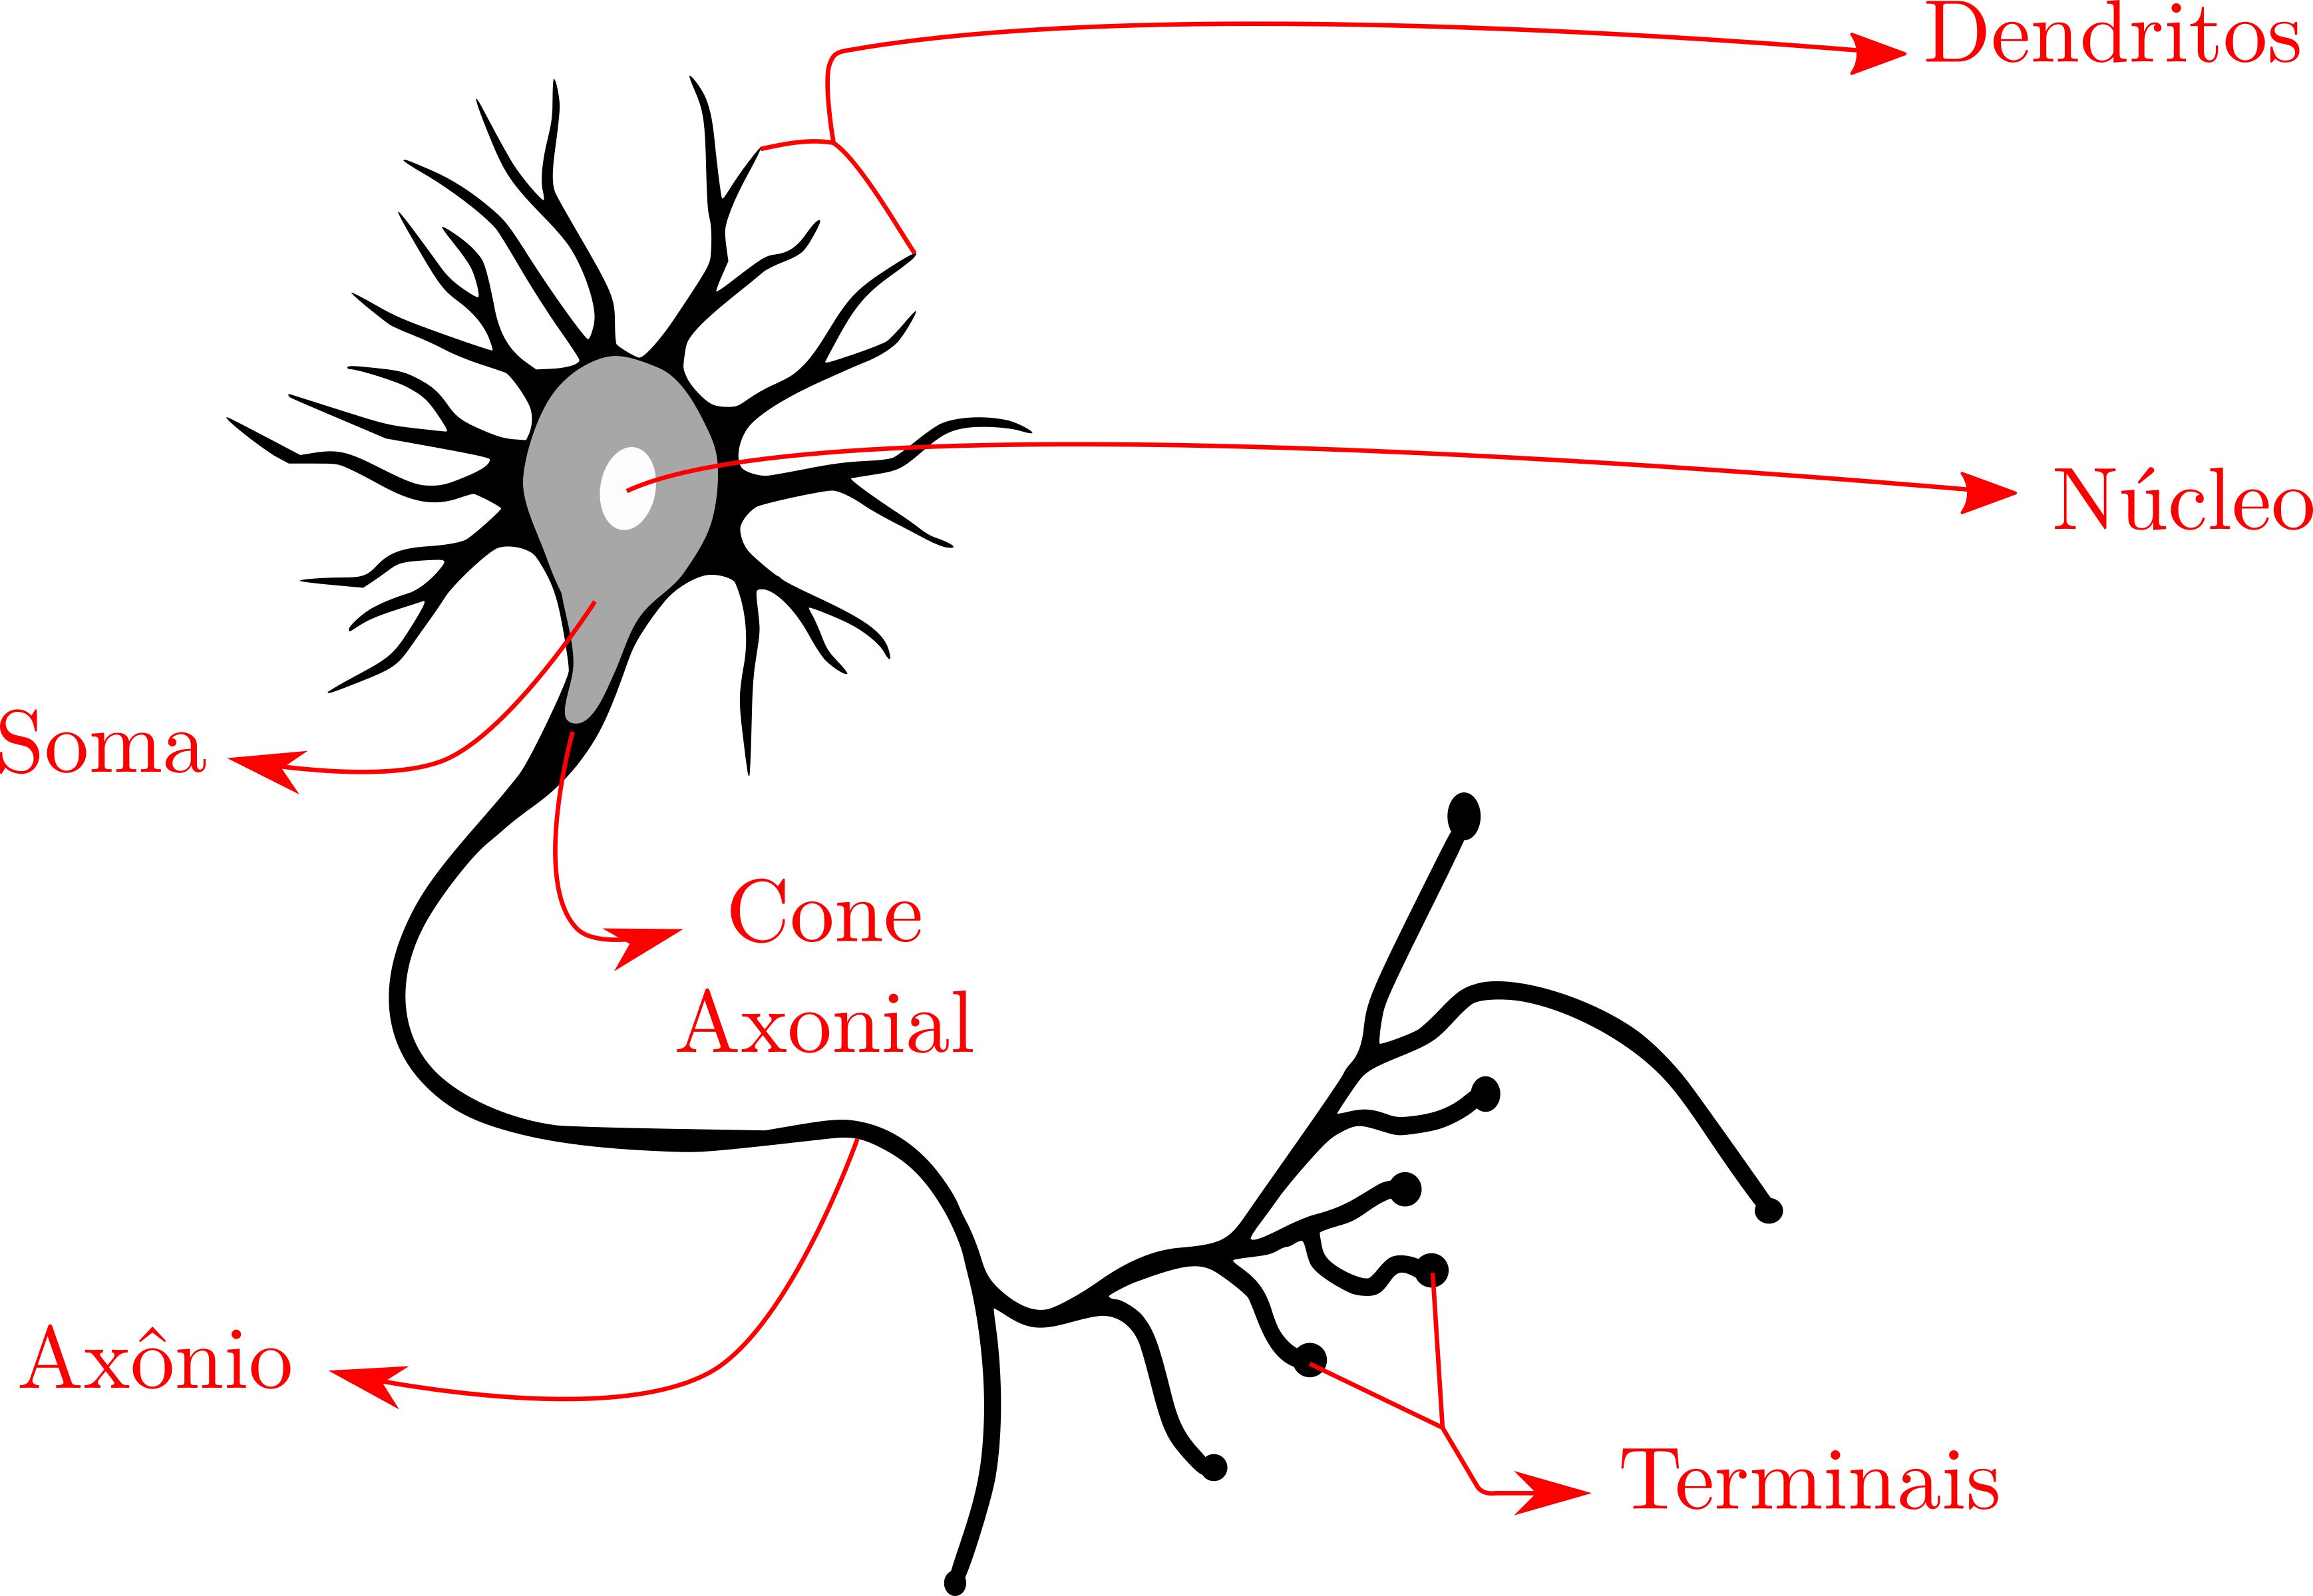
\includegraphics[width=0.7\textwidth]{Imagens/Fig3.png}
	\caption{Neurônio esquemático com suas subdivisões.}
\end{figure}

O caminho do impulso elétrico se dá por meio destas unidades celulares interconectadas, os neurônios, através de sua membrana celular. Um neurônio, em estado de repouso, apresenta carga elétrica positiva, no lado externo. E carga negativa no lado interno. Esta situação é denominada estado de \textit{Polarização}. Esses íons são principalmente sódio ($Na^{+}$), cloro ($Cl^{-}$), potássio ($K^{+}$) e cálcio $(Ca^{2+}$) e deslocam-se através de canais proteicos inseridos na bicamada fosfolipídica da membrana plasmática do neurônio \citep{impulso2016}. A diferença entre essas cargas é mantida por um sistema denominado \textit{Bomba de íons}\footnote{Tal mecanismo regula as trocas iônicas no espaço entre dois neurônios e reverte a polaridade da membrana celular no momento da passagem do impulso elétrico.}.

O sistema é acionado quando um estímulo externo, de origem química, mecânico ou até mesmo elétrico, chega ao neurônio perturbando a condição de equilíbrio da Bomba de Sódio e Potássio, permitindo a entrada de uma grande quantidade de sódio e uma pequena quantidade de potássio. Caso o valor crítico seja ultrapassado o potencial passa de repouso para ação. 

Imediatamente após a passagem do impulso nervoso, a membrana sofre repolarização, recuperando o seu estado de repouso. 

\begin{figure}[H]
	\centering
	
\includegraphics[width=0.7\textwidth]{Imagens/Fig4.png}
	\caption{Conjuntos de lipídeos chamados canais iônicos abrem "portas" que deixam passar íons, por meio de substâncias susceptíveis à campos elétricos, que por sua vez são estimulados por correntes elétricas. Esse procedimento gera uma DDP  que realiza a transmissão do sinal \citep{Kandel2000}.}
\end{figure}

Analogamente a RNA faz uma representação simplista dos processos físico-químicos destas neurosubstâncias, por $\omega_{i,j}$. 

\begin{figure}[H]
	\centering
	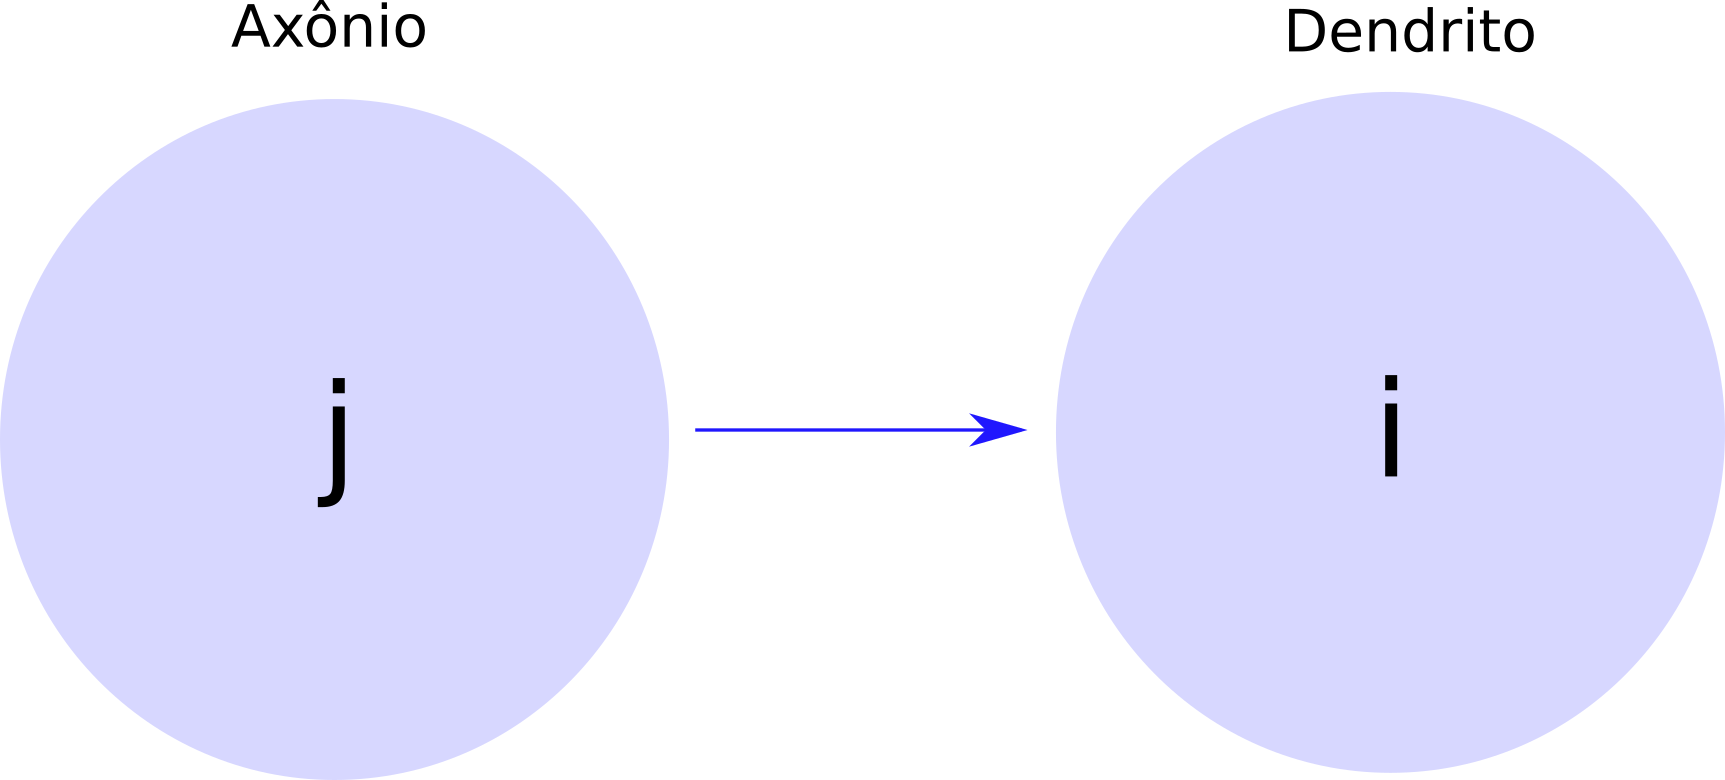
\includegraphics[width=0.7\textwidth]{Imagens/Fig5.png}
	\caption{Direção e sentido de um impulso nervoso em uma RNA. A seta azul indica o sentido do movimento que vai do índice $j$ para o índice $i$.}
\end{figure} 

As neurossubstâncias são divididas a saber:

\begin{enumerate}
	\item neurotransmissores: são substâncias que são transmitidas no espaço entre dois neurônios e atuam em um curto intervalo de tempo.
	\item neuromoduladores: alteram a capacidade de transmissão da informação de longo prazo.
\end{enumerate}


O parâmetro do modelo é chamado de peso sináptico. Ele é descrito como $\omega_{j,i}$ onde $j$ é a origem e $i$ o destino.

\begin{figure}[H]
	\centering
	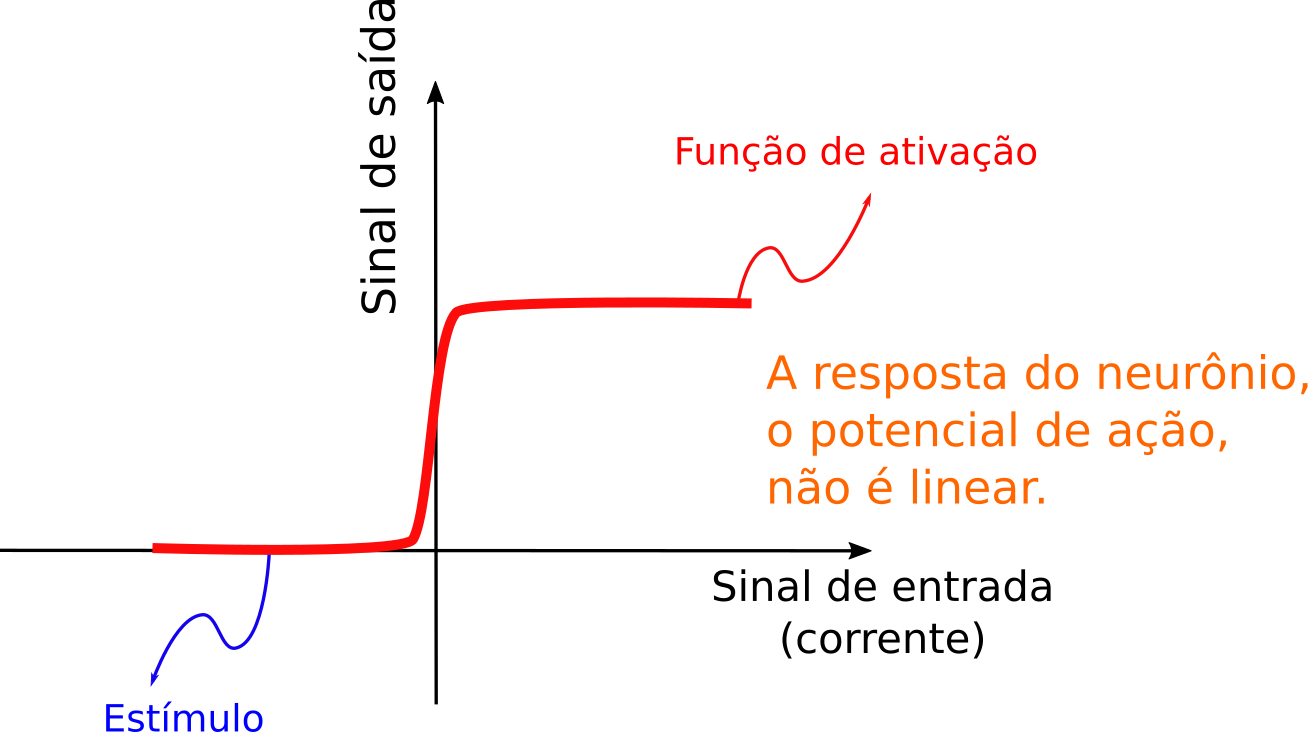
\includegraphics[width=0.7\textwidth]{Imagens/Fig6.png}
	\caption{Função de ativação em um neurônio.}
\end{figure} 

A representação dinâmica do sistema é ma função não-linear e não-periódica.


\begin{figure}[H]
	\centering
	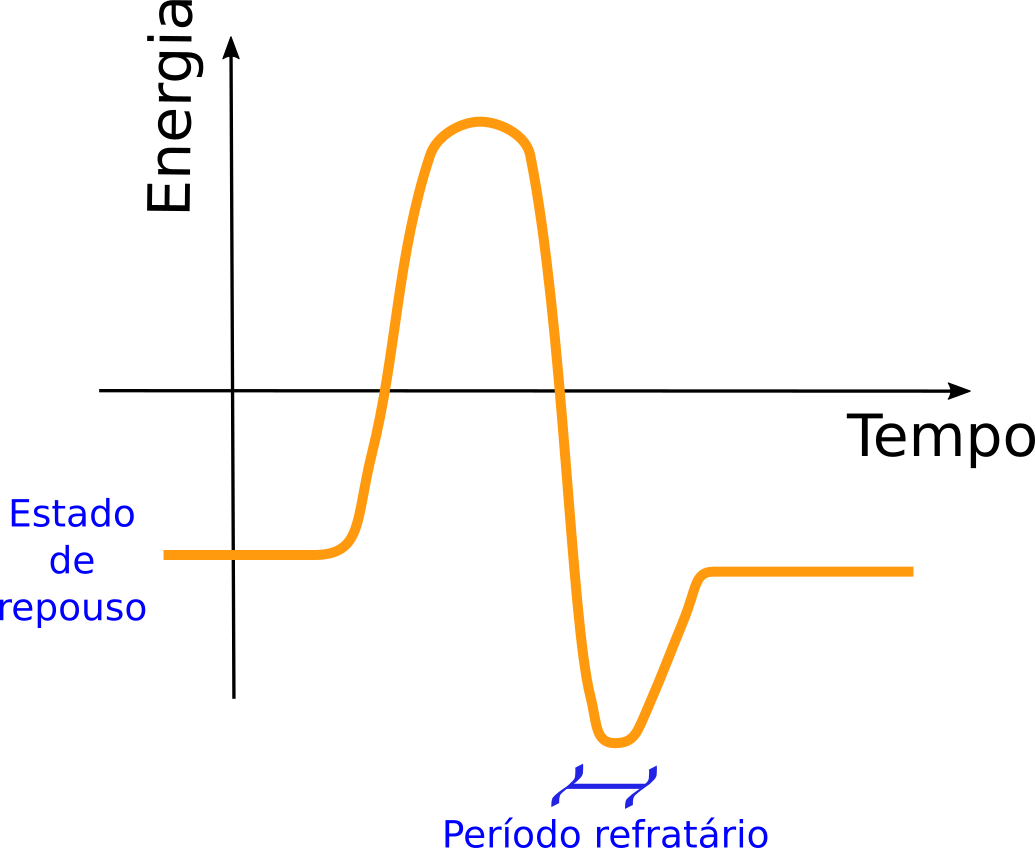
\includegraphics[width=0.5\textwidth]{Imagens/Fig7.png}
	\caption{Representação dinâmica do sistema.}
\end{figure} 

Ao término do período refratário (contado após o disparo)a célula está pronta para receber um novo estímulo.


\subsection{O modelo computacional de um neurônio}

Em termos de ciência da computação o cérebro pode ser descrito como um sistema paralelo com cerca de $10^{11}$ processadores. De acordo com a figura \ref{MCN} cada processador computa uma soma ponderada dos dados de entrada que vêm de outros processadores. E a saída é um único número que é a imagem de função não linear, que pode ser uma tangente hiperbólica ou uma função degrau \footnote{Esta função é chamada de função de ativação}. 

\begin{figure}[H]
	\centering
	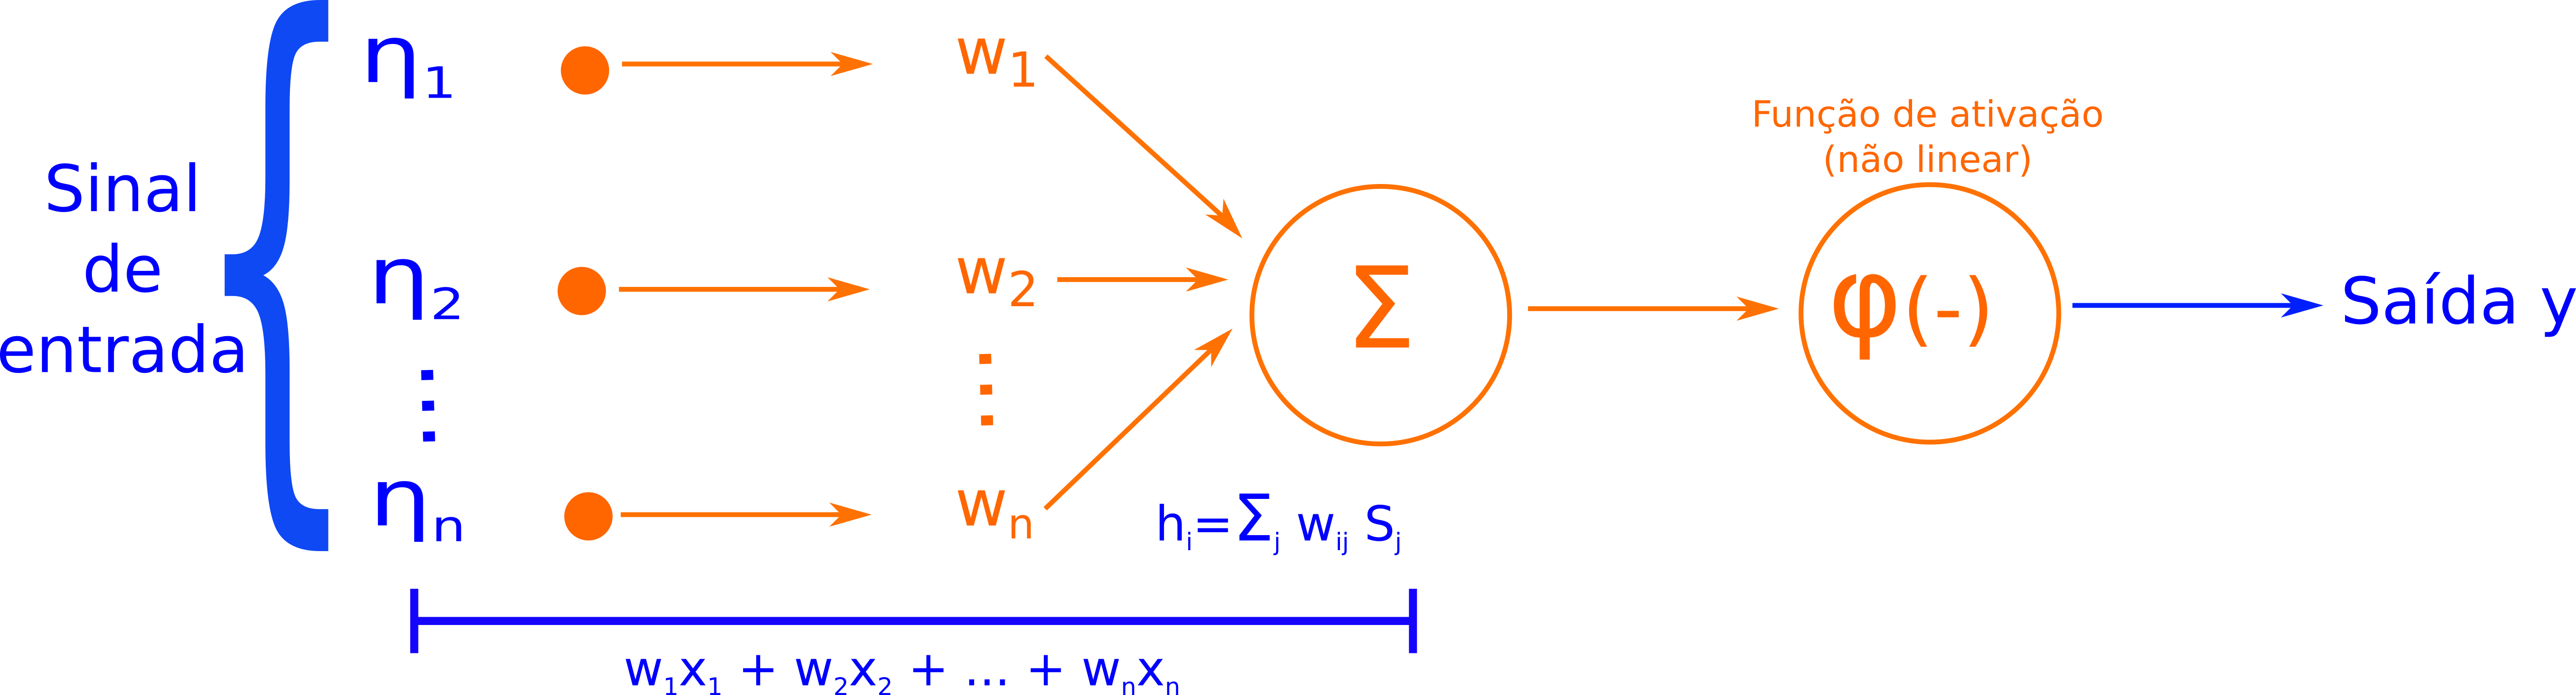
\includegraphics[width=1.2\textwidth]{Imagens/Fig8.png}
	\caption{Soma ponderada dos pesos sinápticos com o sinal de entrada}
	\label{MCN}
\end{figure} 

A alta conectividade entre da rede, o que se verifica no número de termos do somatório, significa que os erros que ocorram em alguns termos terão pouca relevância no cômputo final do sinal de saída.  

\subsection{Histórico}

As ideias utilizadas na psicologia datam da época de Aristóteles. Contudo a base computacional da modelagem neuronal é traçada a partir do artigo de \citet{McCulloch1943}. 

Durante os $15$ anos seguintes este trabalho se configurou como um marco no detalhamento da lógica dos limiares de ativação das redes neuronais. Ele era capaz de realizar uma computação considerada universal e eram consideradas como máquinas de estados finitos \citep{Misky1969}. 

Na década de $60$, o foco dos estudos utilizando redes neuronais estava em como achar o peso apropriados $w_{ij}$ para tarefas computacionais específicas \citep{Rosenblatt1962}. O grupo de \citet{Rosenblatt1962} concentrou esforços no modelo denominado de \textbf{perceptrons}, que foram organizados em camadas unidirecionais entre a camada anterior e a posterior \citep{Hertz1990}.


O neurônio de \citet{McCulloch1943} propõe um limite binário para a criação de um modelo. Este neurônio artificial registra uma soma de pesos de $n$ sinais de entrada, $\eta_{i}$, $i=1,2,3,...,n$, e fornece um \textit{output}\footnote{Valor de saída} de $1$ caso esta soma esteja acima do limite $\mu_{i}$. Caso contrário o \textit{output} é $0$. Matematicamente essa relação de evolução temporal do sistema pode ser descrita de acordo com a Eq. \ref{Eq.neuronio-McCulloch}:

\begin{eqnarray}
\eta_{i}(t+1)=\Theta \left( \sum^{n}_{i=1} w_{ij} \eta_{i}(t) -\mu_{i} \right)
\label{Eq.neuronio-McCulloch}
\end{eqnarray}



Onde $\Theta$ é o passo dado na posição $0$, $w_{ij}$ é chamada sinapse-peso associado a um $i_{esimo}$ \textit{input}. A título de simplificação a função limite\footnote{Genericamente chamada de função de ativação} $\mu_{i}$ é considerada um outro peso $w_{0}=-u$ anexado a um neurônio com um \textit{input} constante $x_{0}=1$. 

Pesos positivos correspondem a uma sinapse \textbf{excitatória}, enquanto pesos negativos correspondem a uma sinapse \textbf{inibitória}. Este modelo contém uma série de simplificações que não refletem o verdadeiro comportamento dos neurônios biológicos \citep{Mao1996}.  

Derivações do neurônio de \citet{McCulloch1943} na escolha das funções de ativação. Uma função largamente utilizada é a função degrau e a função sigmóide, que exibe uma suavização dos \textit{outputs} a medida que o valor da função diminui \citep{Mao1996,Misra2010}. Essa função de ativação pode ser expressa de acordo com a Eq. \ref{f.sigmoide}:

\begin{eqnarray}
g(x)=1/(1+e^{-\beta x})
\label{f.sigmoide}
\end{eqnarray}

Onde $\beta$ é o parâmetro de inclinação. A Fig. \ref{Esquematico de McCulloch} ilustra a sequência lógica da operação de uma RNA para um neurônio simples de McCulloch-Pitts. 
\\
\begin{figure}[H]
	\centering
		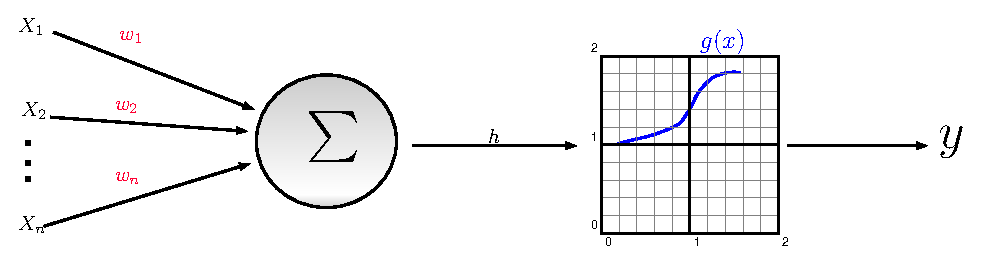
\includegraphics[scale=0.7]{Imagens/McCulloch.eps}
	\caption{Modelo esquemático de um neurônio de McCulloch-Pitts. Onde $x_{1}, x_{2}, ..., x_{n}$ são os \textit{inputs}, $w_{1}, w_{2}, ..., w_{n}$ são os pesos, h é o treino, $g(x)$ é a função de ativação, e $y$ é o \textit{output}.}
	\label{Esquematico de McCulloch}
\end{figure}

Mais de $50$ tipos de redes neuronais artificiais tem sido criadas até o ano de $2014$ \citep{Saljooghi2014}.

\subsection{O modelo de McCulloch-Pitts ($1943$)}
Foram os primeiros a modelar matematicamente um neurônio

\begin{eqnarray}
\centering
h_{i}(t)= \sum_{j} \omega_{i,j} \eta_{j}(t)
\end{eqnarray}

A função de movimento dentro deste modelo é dada por:

\begin{eqnarray}
\centering
\eta_{i}(t+1)= \Theta(h_{i}-\mu_{i})
\end{eqnarray}

Onde o $\theta$ é a função degrau, $h_{i}$ é o estado do neurônio e $\mu_{i}$ é o limiar de ativação. A função degrau possui dois argumentos é pode ser definida como;

\begin{eqnarray}
\centering
\Theta(x)=
\begin{cases}
1,\; se\; x>0 \\ 
0, \text{caso contrário}
\end{cases}
\end{eqnarray}


\begin{figure}[H]
	\centering
	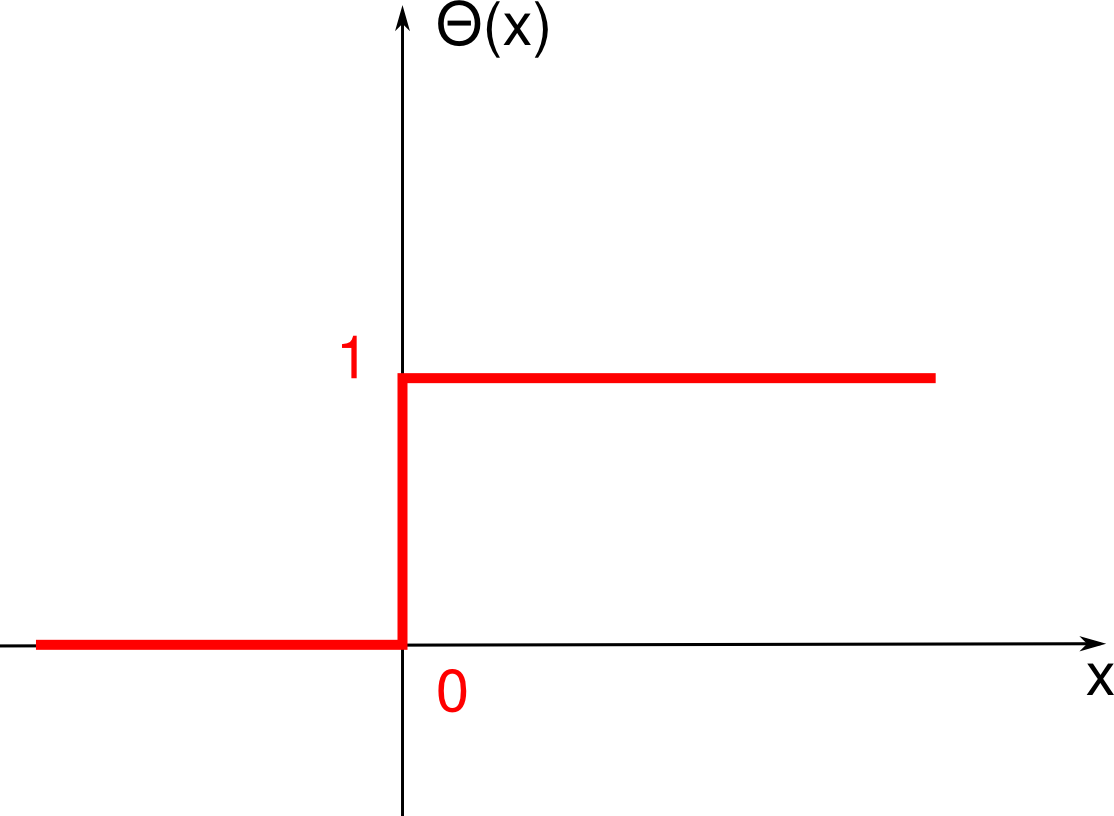
\includegraphics[width=0.5\textwidth]{Imagens/Fig9.png}
	\caption{Função de ativação.}
	\label{Degrau}
\end{figure} 

O $\mu_{i}$ vai controlar o ponto de descontinuidade da função.


\begin{figure}[H]
	\centering
	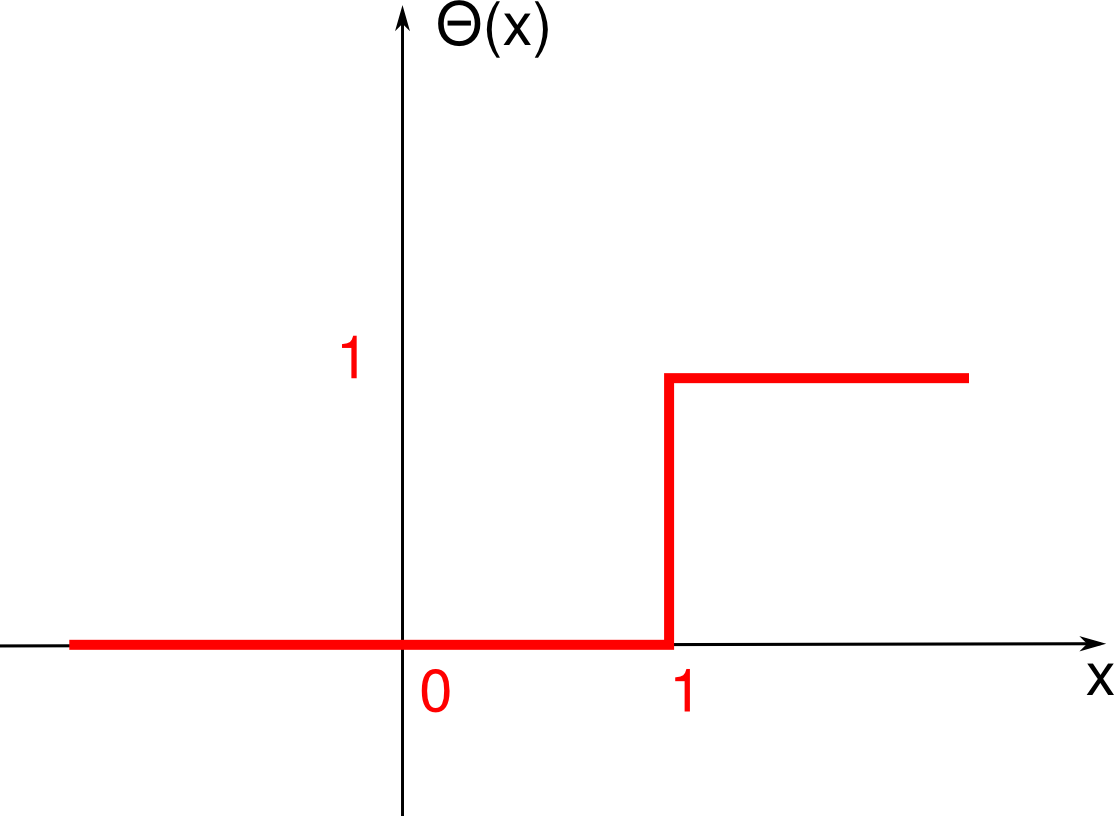
\includegraphics[width=0.5\textwidth]{Imagens/Fig10.png}
	\caption{Função de ativação com o argumento contrário alterado para $1$.}
	\label{Degrau2}
\end{figure} 


\begin{eqnarray}
\centering
\eta_{i}(t+1)= \Theta\left( \underbrace{\sum \omega_{i,j}\; \eta_{j}(t)}_{h_{i}}\;-\;\mu_{i}\right)
\label{movimento}
\end{eqnarray}

Quando $\omega_{i,j}$ é positivo denominamos a sinapse de \textit{excitatória} e $\omega_{i,j}$ é negativo denominamos a sinapse de \textit{inibitória}. As somas ponderadas devem atingir ou exceder o $\omega_{i}$ para um neurônio disparar.

Leitura recomendada: Wedemann,R., Avalanche: Pysica A. 

\subsection{Modelo Matemático Simples Não-linear}

\citet{McCulloch1943} provaram que uma assembleia síncrona é capaz de realizar comutação universal. ou seja, dependendo da topologia do grafo orientado completamente conexo você será capaz de solucionar qualquer tipo de função. 

Uma topologia pode ser definida por meio de um grafo pelos seguintes itens: vértices, arestas e pesos. Um simples exemplo de uma topologia pode é dado a seguir:

\begin{itemize}
	\item vértices = [1,2,3]
	\item arestas = [(2,1),(1,3)]
	\item $\omega_{pesos} = [\omega_{1,2},\omega_{3,1}]$
\end{itemize}

\begin{figure}[H]
	\centering
	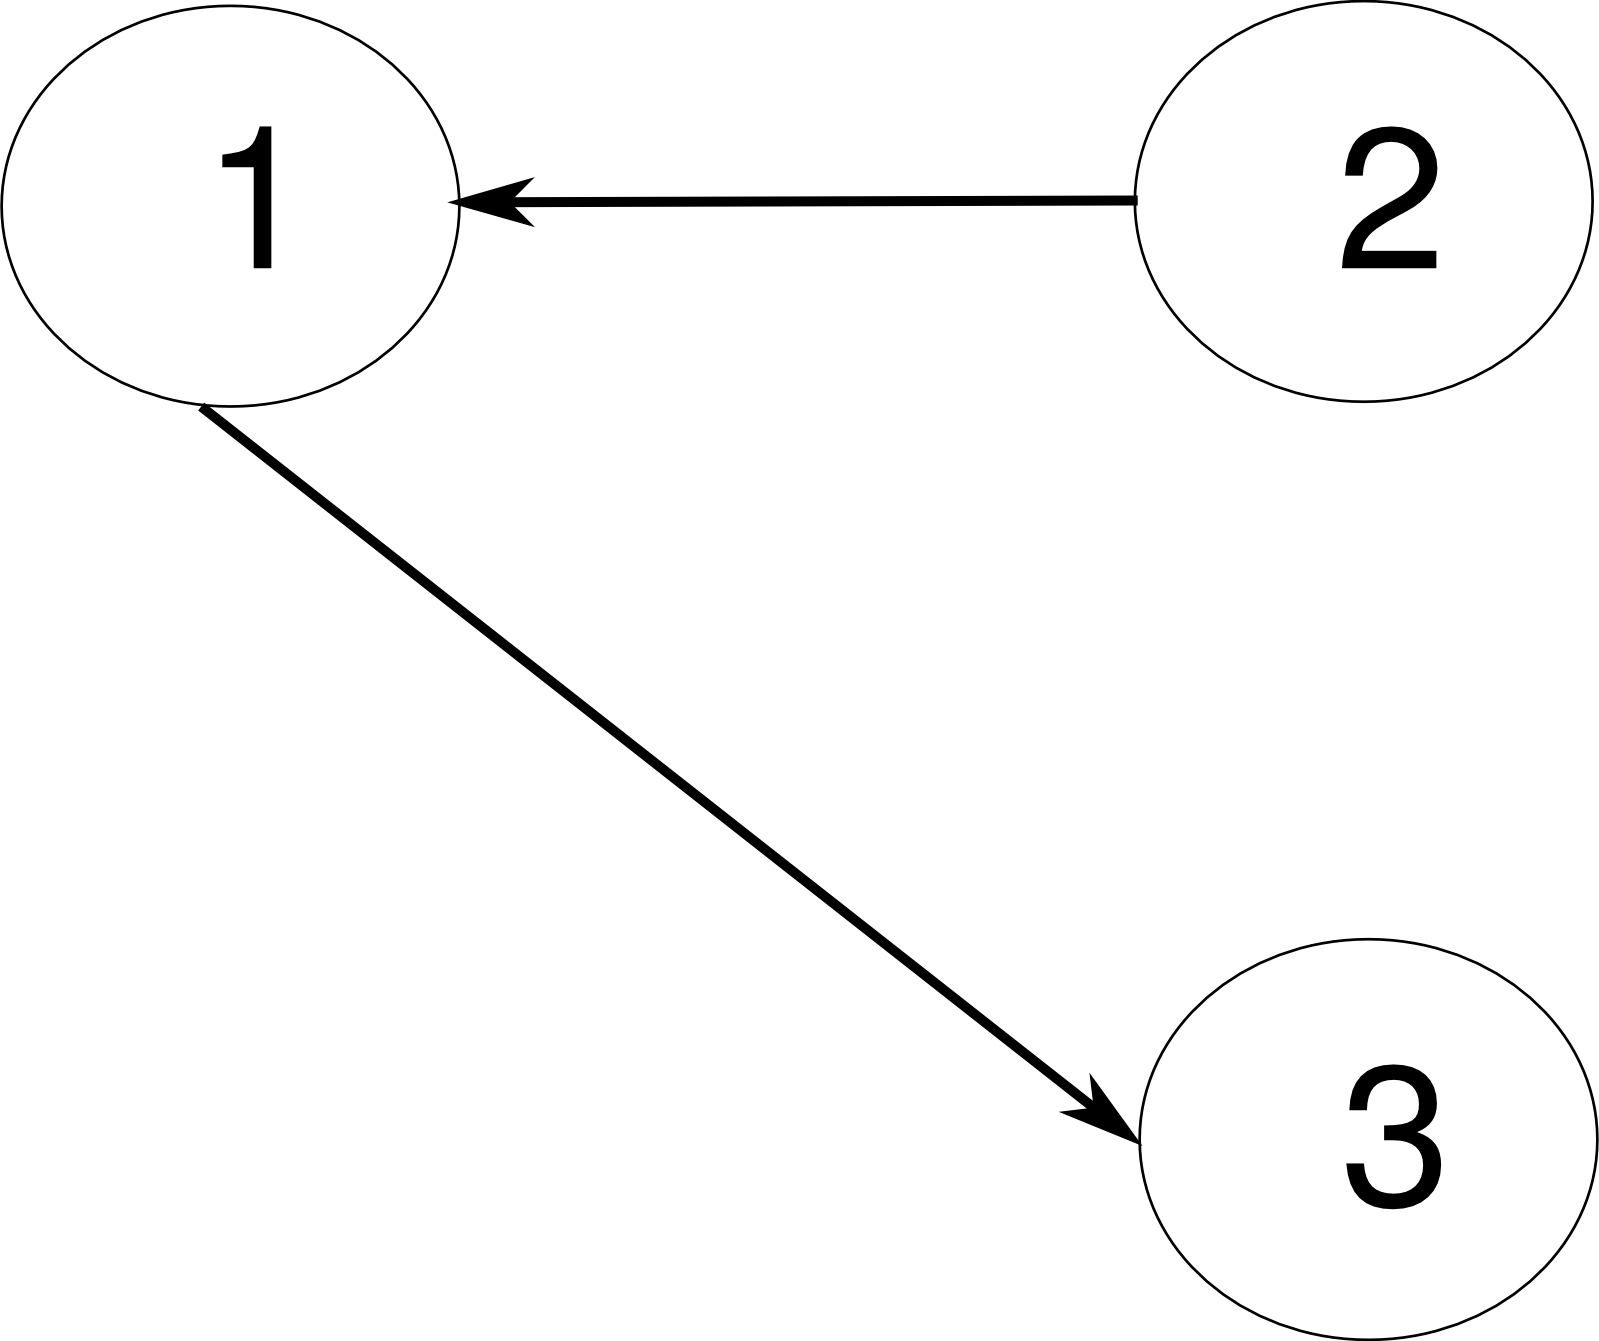
\includegraphics[width=0.5\textwidth]{Imagens/Fig11.png}
	\caption{Topologia de uma rede simples de três neurônios.}
	\label{Topologia}
\end{figure}

A saída é proporcional a entrada da rede. E esta, por sua vez, é ponderada simulando desta forma o que as células reais fazem, de acordo com $h_{i}=\omega_{i,j}\eta_{j}$.

Um neurônio real produz uma sequência de pulsos. Os modelos que se aproximam dessa realidade são chamados de \textit{Spiking Neural Network}.


\section{Terceira aula: 23/08/2017}

O estado de um neurônio pode ser definido como a intensidade do seu sinal, através da equação do movimento (Eq. \ref{movimento}).

\begin{eqnarray}
\centering
\eta_{i}(t+1)= \Theta\left( \underbrace{\sum \omega_{i,j}\; \eta_{j}(t)}_{h_{i}}\;-\;\mu_{i}\right)
\label{movimento}
\end{eqnarray}


\begin{figure}[H]
\centering
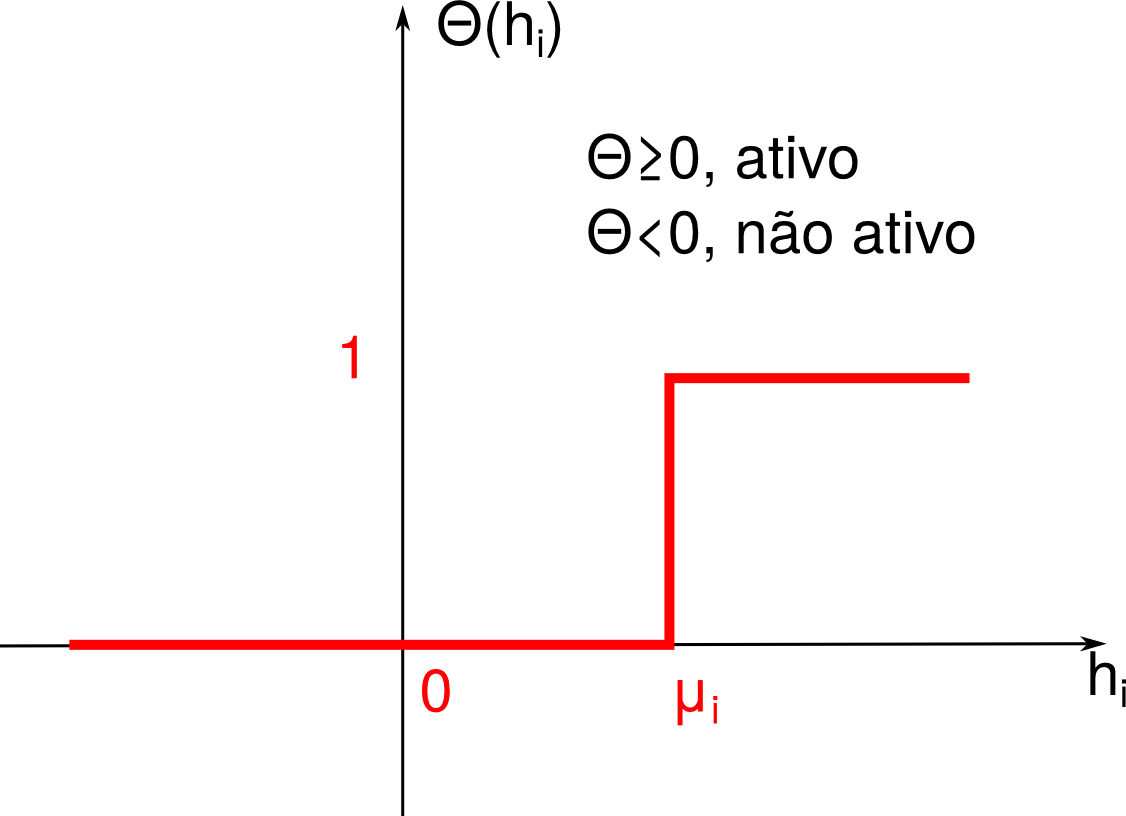
\includegraphics[width=0.5\textwidth]{Imagens/Fig12.png}
\caption{Limites de ativação da sinapse ou \textit{threshold}.}
\label{Ativacao}
\end{figure}

Onde $\Theta$ é a função degrau discreta no ponto $\mu_{i}$ tende ao infinito. 

\begin{eqnarray}
\eta_{i}\coloneqq g\left(\sum_{j} \omega_{i,j} \eta_{j}-\mu_{i}\right)
\end{eqnarray}
	
Em algoritmos o sinal de atribuição diz que a variável $\eta_{i}$ assumirá os valores de g (função de ativação, que dá a mudança de estado da rede). Onde $\eta_{i}$ é chamado de estado.

O tempo que a informação leva para ser transferida pode ser modelada de maneira síncrona ou assíncrona. Este princípio pe chamado detecção de neurônios dependentes. 

\begin{figure}[H]
\centering
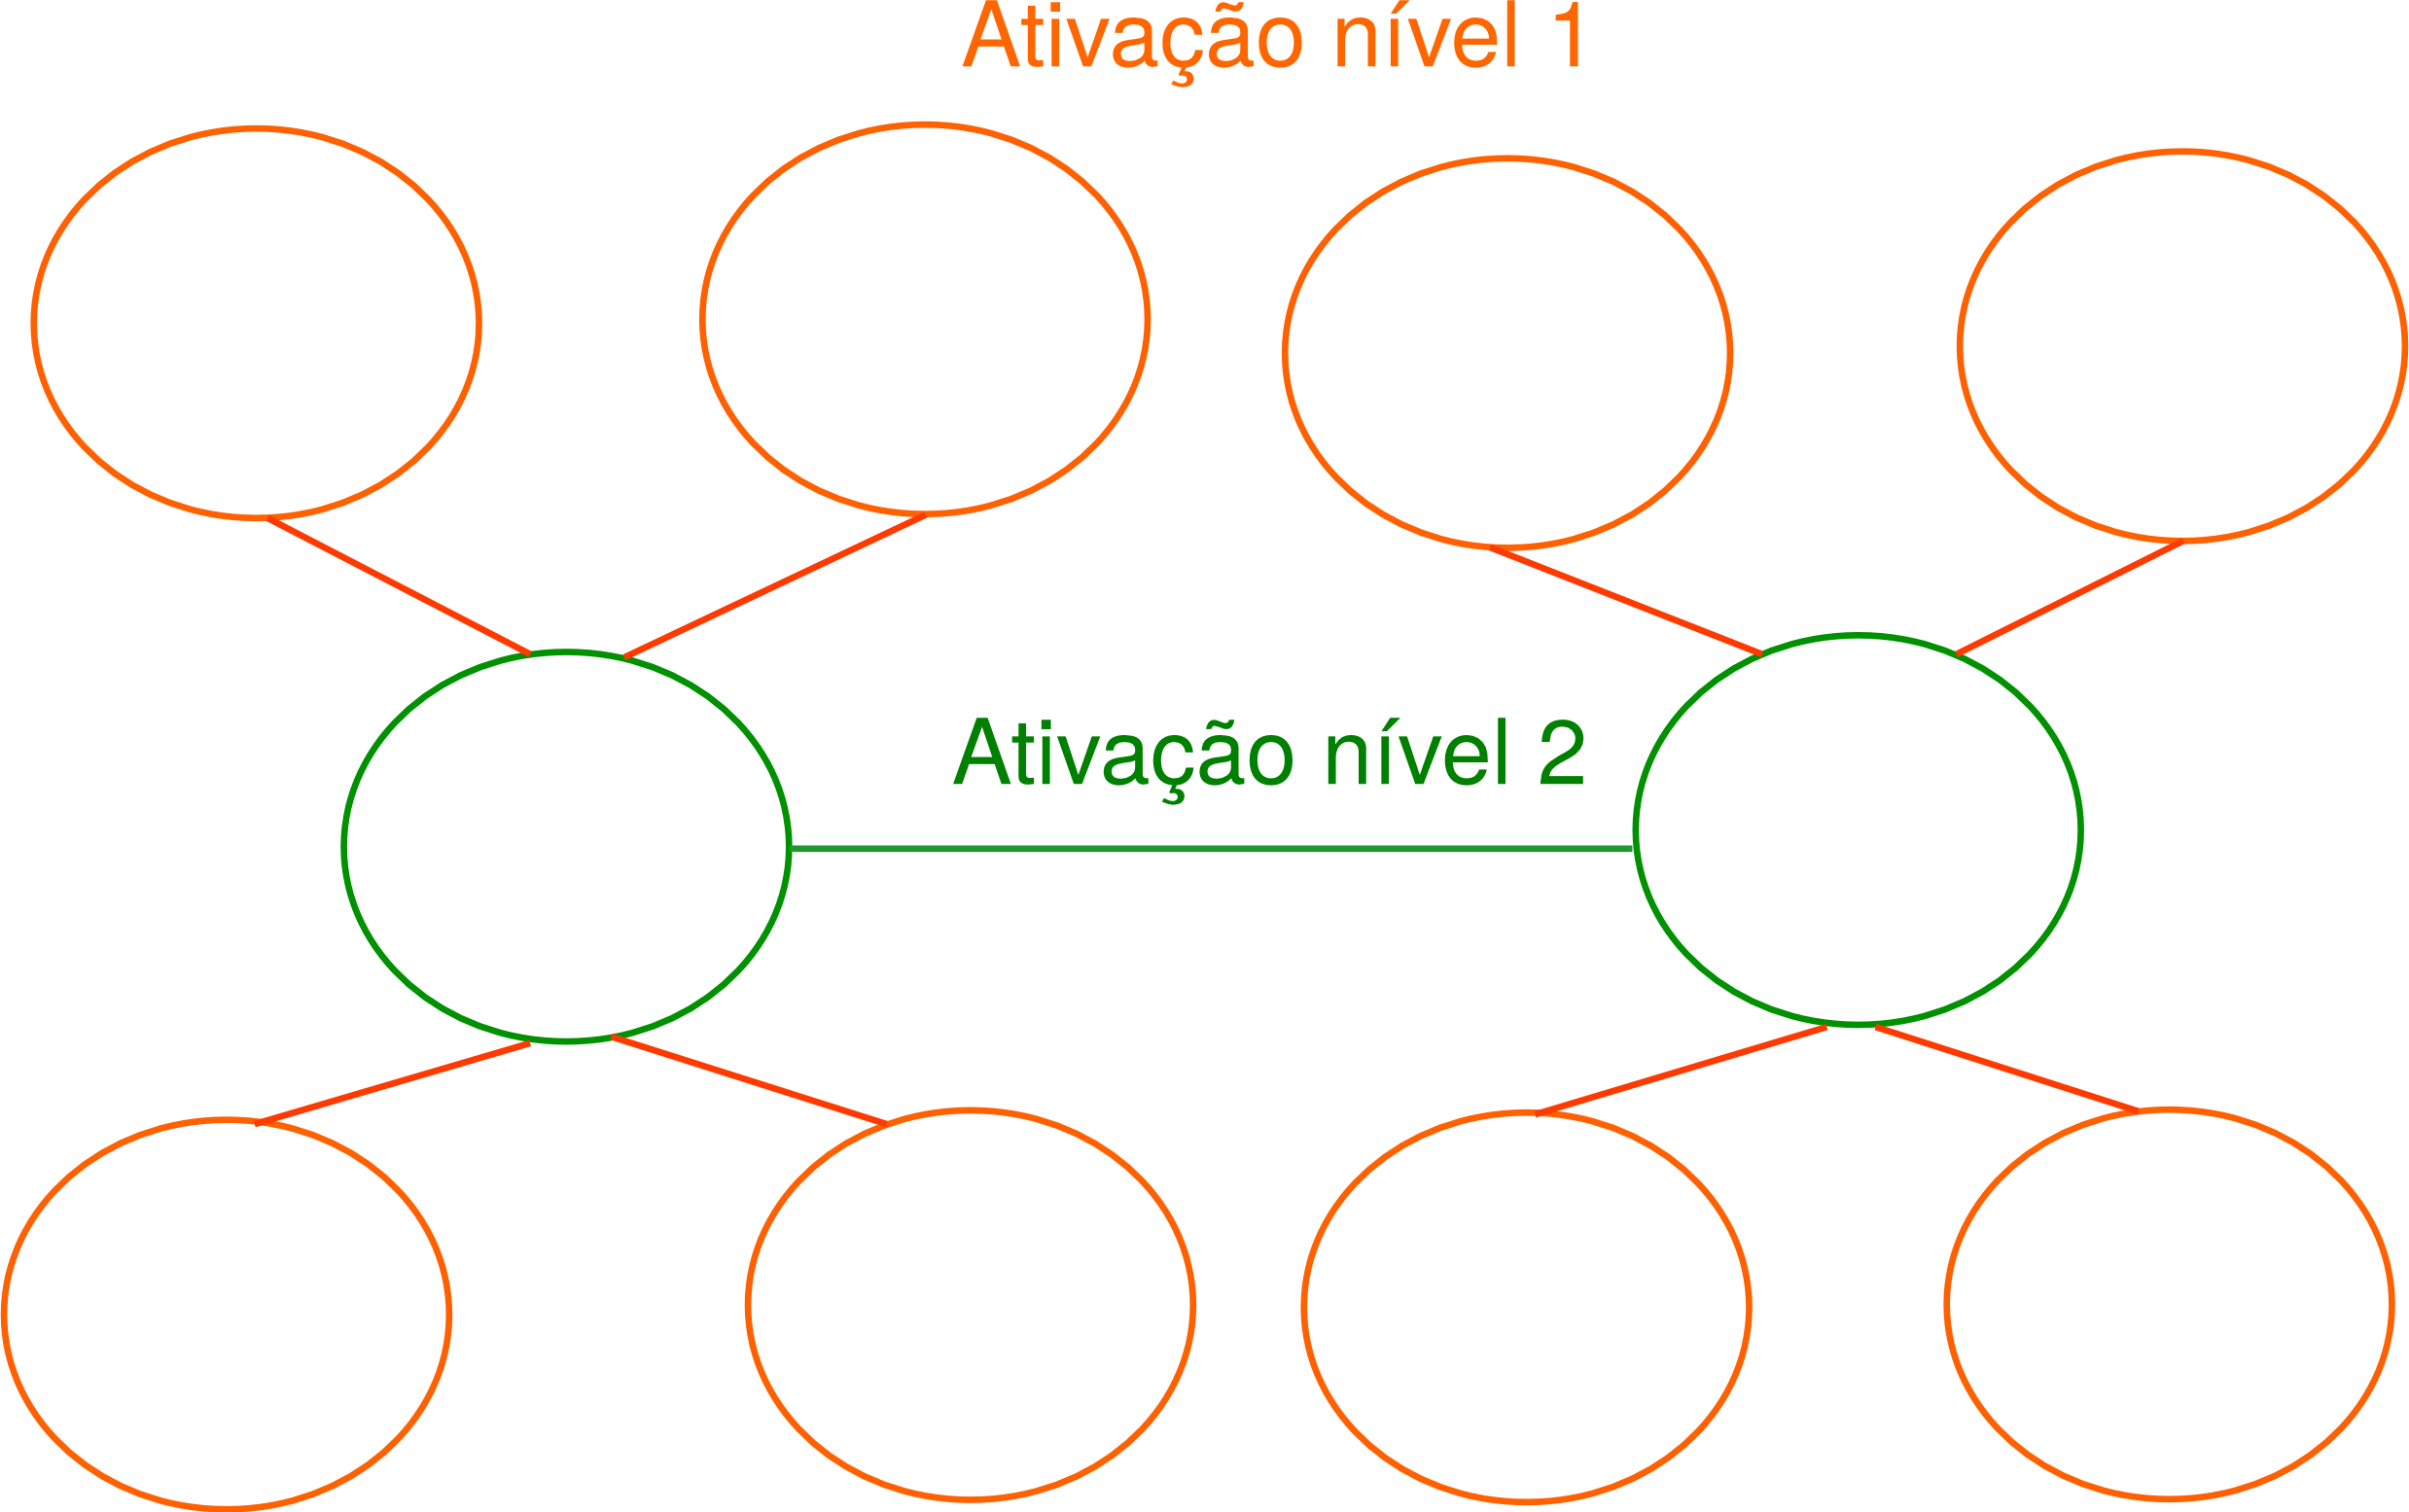
\includegraphics[width=1\textwidth]{Imagens/Fig13.png}
\caption{Níveis diferentes de ativação em uma topologia neuronal.}
\label{Ativacao}
\end{figure}

Em algoritmos sequenciais a atualização não é síncrona. 

\subsection{Como se mapeia o caminho do sinal na rede?}

O caminho é uma função do estado do neurônio em relação ao tempo. O estado da rede, portanto, é um conjunto ($\eta_{1},\eta_{2},\eta_{3}$), ou seja dos estados dos neurônios.  

\begin{figure}[H]
	\centering
	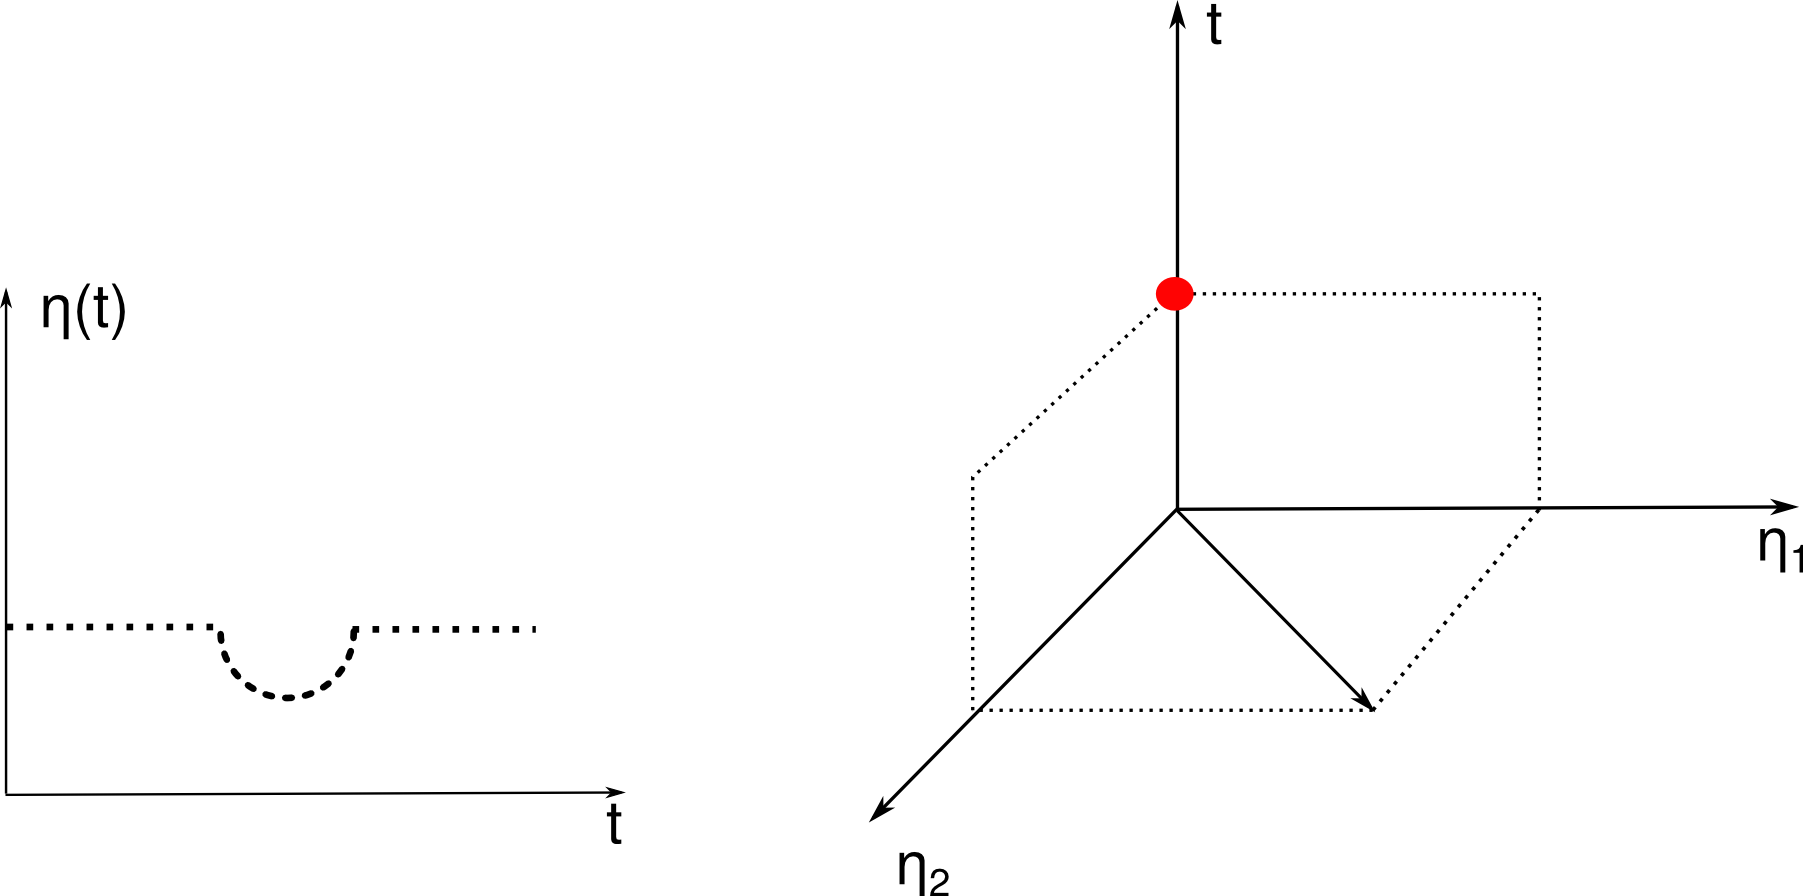
\includegraphics[width=1\textwidth]{Imagens/Fig14.png}
	\caption{Estado de uma rede em função de $\eta(t)$ para os conjuntos $(\eta_{1},\eta_{2})$.}
	\label{tempo}
\end{figure}

Como dito anteriormente representam-se uma rede através de grafos. E quando estes possuem somente uma direção entre os estados dos neurônios, eles são chamados de \textit{Feedfoward network}. Quando estas são ligadas entre os estados através de laços entres os neurônios, ou seja, com dois sentidos entre eles, estas são chamadas de \textit{Bi-directional network}.

Nas RNA's modelos de neurônios são chamados de unidade de processamento, enquanto que as sinapses são tratadas como pesos ou conexões. Uma rede pode ser dita como robusta se o sistema não se degrada com a retirada de neurônios. Por conseguinte afirma-se que esta tem a capacidade de se adaptar aos ruídos do meio. 

\section{Quarta aula: 04/10/2017}

	Recapitulando o modelo de \citet{McCulloch1943} temos:
	
\begin{enumerate}
	\item $\eta_{i}(t+1)= \Theta\left( \underbrace{\sum \omega_{i,j}\; \eta_{j}(t)}_{h_{i}}\;-\;\mu_{i}\right)$
	\item $h_{i}=\sum_{j\in \text{vizinhanças}}=\omega_{i,j} \eta_{j}(t)$
	\item $\eta_{i}(t+1)= \Theta \left(h_{i}-\mu_{i}\right)$
\end{enumerate}

  Onde $1$ é a equação de movimento, $2$ é o estado do neurônio, $3$ é a equação reduzida de movimento com o limiar de ativação $\mu_{i}$.

\begin{figure}[H]
	\centering
	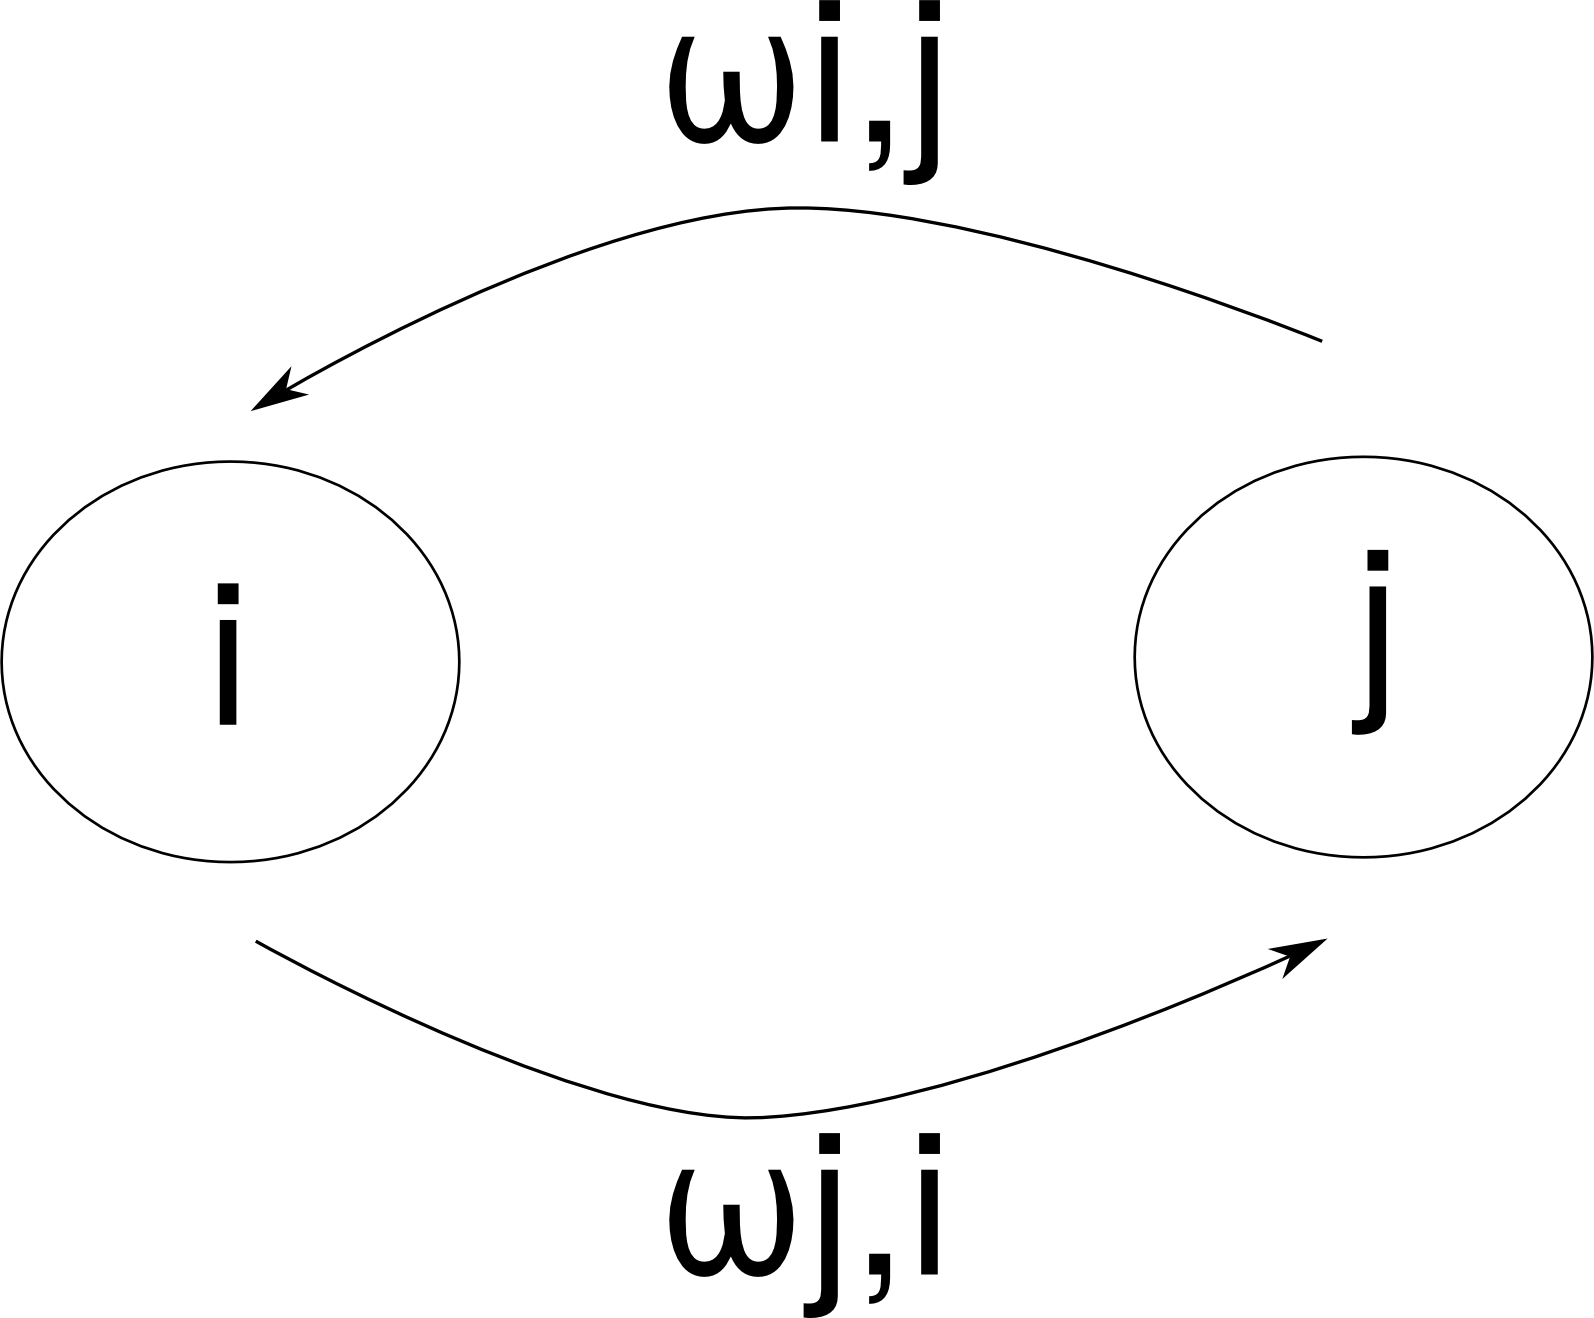
\includegraphics[width=0.5\textwidth]{Imagens/Fig15.png}
	\caption{Orientação dos pesos entre dois neurônios i e j.}
	\label{tempo}
\end{figure}
   
O $\Theta$ que por padrão é descrito pela função degrau pode ser substituído por modelos contínuos. Os exemplos muito comuns utilizados são as funções sigmoide (Eq.\ref{sig}) e a tangente hiperbólica (Eq.\ref{hip}).
\begin{eqnarray}
\dfrac{1}{1+e^{-\beta(h_{i}-\mu_{i})}}
\label{sig}	
\end{eqnarray}

\begin{figure}[H]
	\centering
	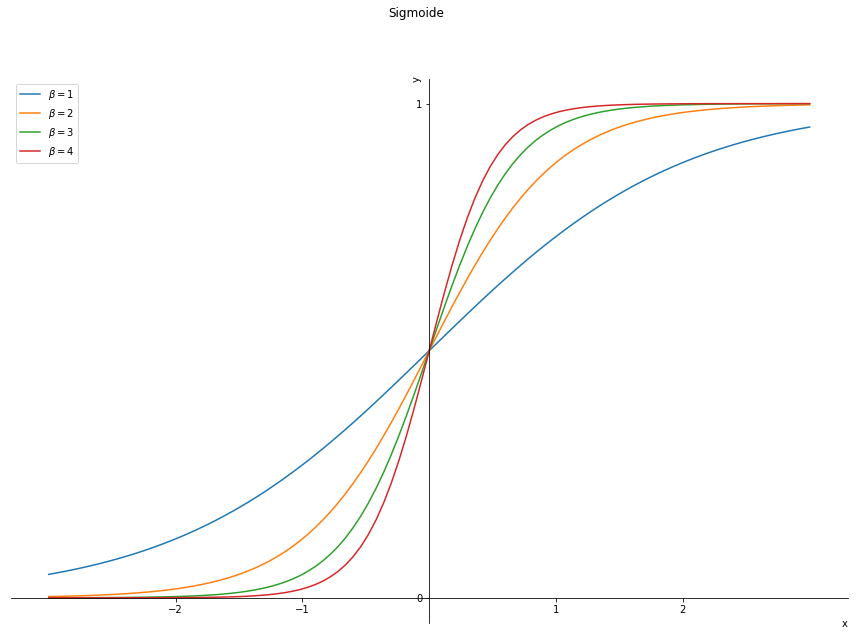
\includegraphics[width=0.5\textwidth]{Imagens/sigmoide.png}
	\caption{Função Sigmoide.}
	\label{HIP}
\end{figure}

\begin{eqnarray}
\tanh(h_{i})
\label{hip}
\end{eqnarray}

\begin{figure}[H]
	\centering
	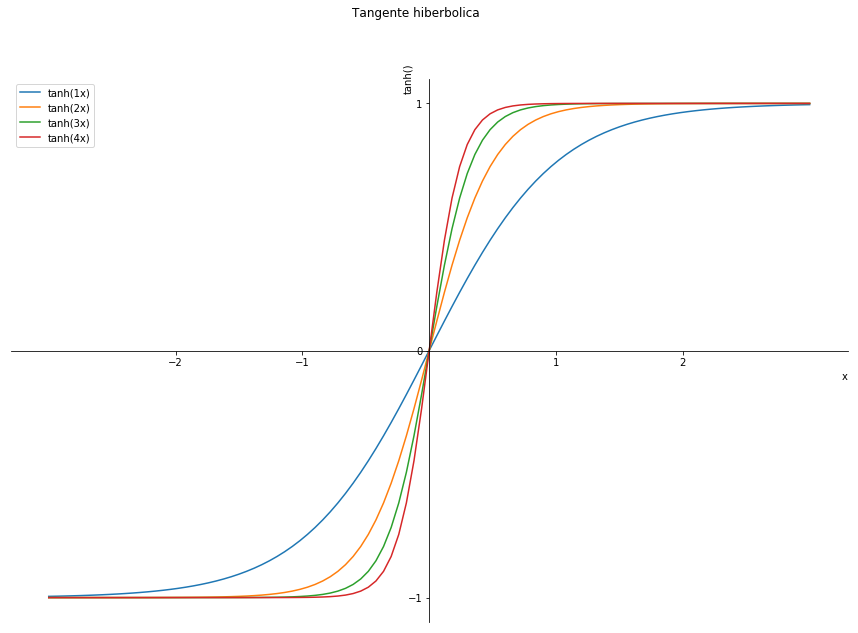
\includegraphics[width=0.5\textwidth]{Imagens/tanh.png}
	\caption{Tangente hiperbólica.}
	\label{HIP}
\end{figure}


Na matemática neuronal as sinapses são chamadas de unidades e as conexões são denominadas de pesos. 

\subsection{O modelo de \citet{Hopfield1982}}

 \citet{Hopfield1982} foi o primeiro a criar um modelo que armazenasse um \textit{memória}. E isso foi feito através do problema da memória associativa onde temos $p$ é o número de padrões armazenados, $n$ é o número de neurônios, $\mu \in \{1,2,3,\hdots, p\}$, e $i \in \{1,2,3,\hdots, n\}$, $\vec{\zeta^{\mu}}$ é o padrão armazenado da rede, $\zeta^{\mu}_{i}$ é um elemento do vetor de padrões armazenados. Sendo assim, para uma rede simples com três neurônios e um padrão armazenado temos:
 
\begin{figure}[H]
	\centering
	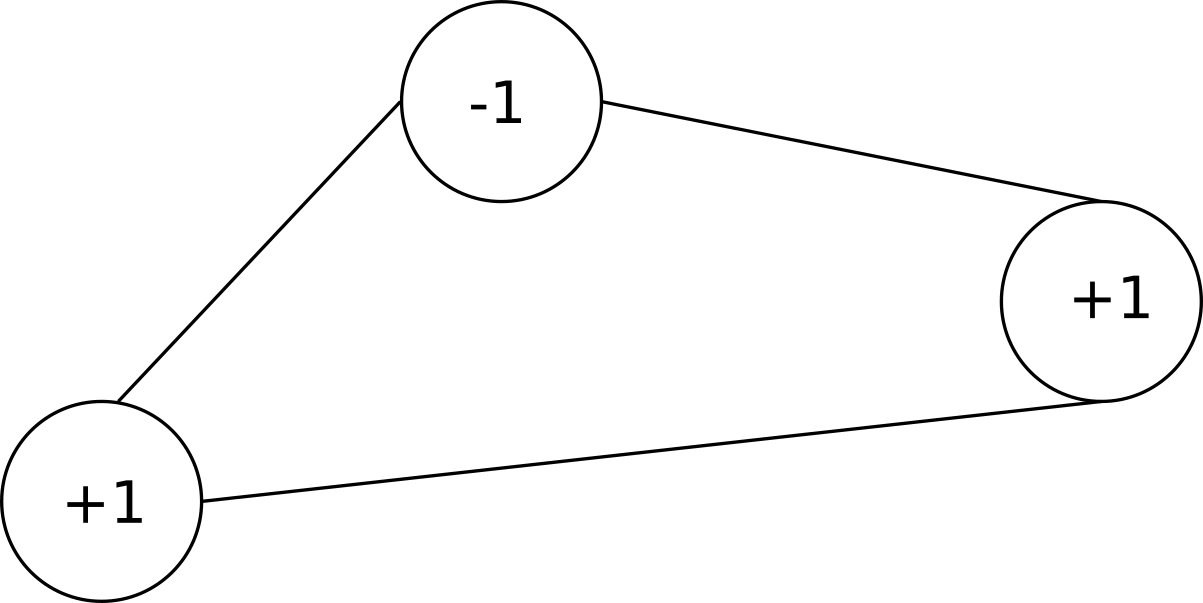
\includegraphics[width=0.5\textwidth]{Imagens/Fig19.png}
	\caption{Podemos escrever um único padrão armazenado como $\vec{\zeta^{1}}=(-1,+1,+1)$}
	\label{1padrao}
\end{figure}

O problema pode ser resolvido através do armazenamento de uma lista de parâmetros por meio do cômputo da distância de \textit{Hamming} que é definida pela equação \ref{hamming}.

\begin{eqnarray}
D_{H} = \sum_{i} [ \zeta^{\mu}_{i} (1-\xi_{i}) + (1 - \zeta^{\mu}_{i}) \xi_{i}]
\label{hamming}
\end{eqnarray}

Onde $\xi_{i}$ é um padrão que se apresenta para a rede. Essa métrica informará o quanto um vetor se distancia do outro.

A memória \textit{associativa}\footnote{A memória associativa também é conhecida como memória não endereçável ou endereçável por conteúdo.} é um processo aonde um dado $\vec{\zeta^{\mu}}$ padrões a rede retornará $\vec{\xi_{k}}$ padrões de saída. A \textit{medida de semelhança} é a menor distância encontrada no cálculo da métrica de Hamming. No caso da memória associativa o padrão armazenado da rede $\vec{\zeta^{\mu}}$ é igual ao padrão apresentado ou padrão de entrada da rede $\xi_{i}$.

\begin{tcolorbox}[colback=green!5,colframe=green!40!black,title=Faça a transformação de variáveis de \ref{ni} para \ref{si}.]
	\begin{eqnarray}
		\eta_{i}(t+1) \coloneqq \Theta\left( \underbrace{\sum \omega_{i,j}\; \eta_{j}(t)}_{h_{i}}\;-\;\mu_{i}\right) 
		\label{ni}
	\end{eqnarray}
	\begin{eqnarray}
	Onde, 
		\Theta(x)=
		\begin{cases}
		1,\; se\; x>0 \\ 
		0, \text{caso contrário}
		\end{cases} \nonumber
	\end{eqnarray}
	\begin{eqnarray}
		S_{i} \coloneqq Sgn (\sum \omega_{ij} S_{j}(t) - \theta_{i} )
		\label{si}
	\end{eqnarray}
	\begin{eqnarray}
	    Onde,
		S_{i}= 2\eta_{i}-1\; e\;  S_{i} \in\{1,-1\} \nonumber
	\end{eqnarray}
	
\end{tcolorbox}



 

%%%%%%%%%%%%%%%%%%%Referências%%%%%%%%%%%%%%%%%
\pagebreak
 \bibliographystyle{apa}
 \bibliography{referencias.bib}

\end{document}